\section{Sensor functionality}

\begin{figure}
    \centering
    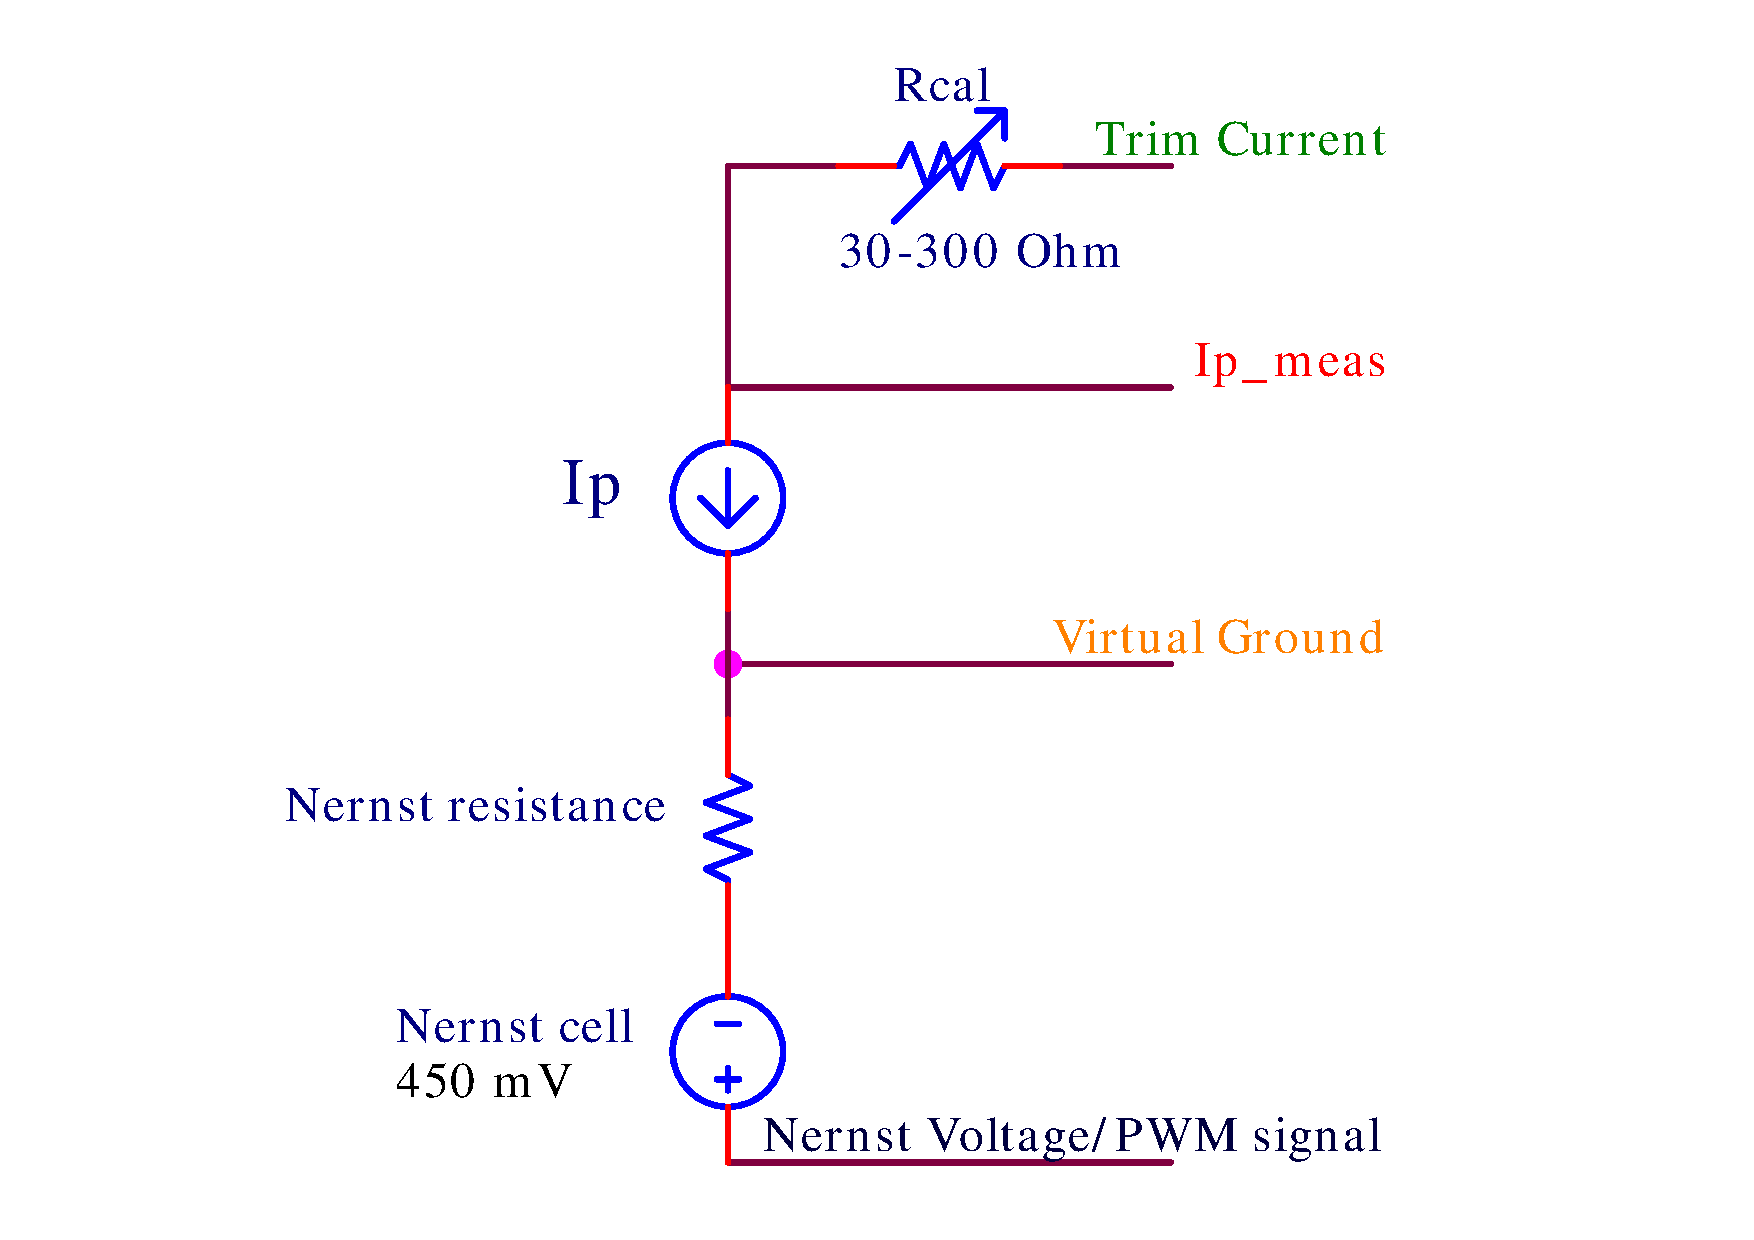
\includegraphics[width = .6\textwidth]{Figures/SCHEMATIC1_lsu49.pdf}
    \caption{BOSCH LSU 4.9 electrical equivalent schematic.}
    \label{fig:schematic_lsu49}
\end{figure}

Figure \ref{fig:schematic_lsu49} shows an equivalent schematic of the oxygen sensor and 4 of its connectors. It does have 6 connectors however, where the 2 connectors which are not shown are for the heating element and is not used in this case. This is because it draws too much current and the sensor is heated up enough by its surroundings in the oven instead.

To control a lambda sensor, its so called nernst voltage has to be held stable at 450 mV relative to its virtual ground, which are both shown in figure \ref{fig:schematic_lsu49}. This voltage is changed depending on the oxygen level and can also be adjusted by the amount of current going through the sensor. Also the amount of current the sensor uses to hold this voltage at 450 mV, tells the lambda value in the air, and from there it is possible to get the oxygen level in the surroundings.


The lambda sensor is a ZrO$_2$ based oxygen sensor, and the nernst voltage builds on the principle discovered by the scientist Walther Nernst~\cite{Exhaust}. The voltage is generated by a partial pressure over a diffusion bar, the voltage occurs from a ionic reaction from the oxygen. This is also why the lambda sensor reacts to other types of substances than oxygen. To assure the sensor only reacts to oxygen, one wants stable substances surrounding the oxygen, like noble gases or nitrogen. When the oxygen is surrounded by more reactable gases like carbon monoxide or hydrogen, it is more likely the lambda sensor gives inaccurate readings~\cite{LSU49}.


But the lambda value varies with the temperature of the sensor and therefore the temperature also has to be calculated. This can be done by sending a \ac{pwm} signal through a known resistance and the nernst cell's resistance to check its impedance by voltage division. Then there is a look up table in the Datasheet \cite{LSU49} to check which resistance corresponds to which temperature. However, when the \ac{pwm} signal is sent through the nernst cell it can't deliver more current than 250 $\mu$A, because of the maximum ratings of the LSU 4.9. Then the voltage drop will most likely be very small within its operating ranges. If this voltage drop would be directly measured by the 10-bit \ac{adc} available on the PIC18F26K22, it would give a bad resolution. To increase this resolution, an instrumental amplifier is used, which amplifies the difference between the \ac{pwm} signal and the signal where the \ac{pwm} signal gets low pass filtered. The gain of the amplifier is then decided to give a good resolution within the operating temperature. Because of this it does not give correct values for lower temperatures, but it should not be a problem because the sensor does not operate correctly in cold temperatures.

The lambda value from the sensor also depends on the pressure from the surroundings. This has to be considered if there is a higher or lower pressure in the oven compared to the atmosphere.

In the datasheet~\cite{LSU49} it is clearly stated that the sensor should be installed within a certain angle to prevent condensation on the sensor, which will prevent accurate readings and also possibilities for damaging the sensor during heat up process. But this sensor is supposed to sit in the exhaust pipe on a car, where it can be a lot of water and high humidity. In this case the sensor will be put in an already preheated oven and therefore it should not be any liquid water that can enter the sensor. Also the most advantageous way to mount the sensor is upwards, because it is mounted in a metal box, with no possibility to mount it on the side or bottom of the box.

%and its position and angle can't be controlled. But because of the very high temperature that occurs in the oven, the possibility for condensation are supposed to be small and therefore the sensors angle hopefully don't have to be considered as much as it would have to be in the exhaust pipe of a car.


\section{Electronic functionality}

In total there will be three differential amplifiers. In this case we use \ac{ic} with pre-built instrumental amplifiers, where you can set the gain with only one resistance. The amplifiers are for the \ac{pwm} signal to measure the temperature, one for measuring the nernst voltage, where it amplifies the 450 mV a few times to reach a higher resolution on our 10-bit \ac{adc} configuration and there is an instrumental amplifier to measure the voltage drop over a 61.9 $\Omega$ resistor to find the $I_p$.


The pump current $I_p$ for the sensor is controlled using a \ac{dac}. The DAC's output is a voltage source, but the resistance after the \ac{dac} is stable and the current is then changed by changing the output voltage from the \ac{dac}. $I_p$ have a low operation swing, and with this follows that the DAC's usable output is about 200 mV. To be able to reach a high-resolution within this output range, one has to select a \ac{dac} with high-resolution itself. The used \ac{dac} is a 12-bit \ac{dac} with \ac{i2c} communication and is an AD5622 \ac{ic} from Analog Devices,~\cite{AD5622}.


By not using the internal heater in the LSU 4.9, there is no need to have access to high voltages and it should make it possible to control the sensor with only 3.3 V. The changes for it to run on 3.3 V, is that the virtual ground has shifted from suggested 2.5 V to about 1.5 V or similar. The important thing is that it is somewhere between 0-3.3 V and that it is possible to reach the wanted voltage ranges from there. In other words high enough to reach the 450 mV over the nernst cell, and low enough so the supply voltage is enough for the pumping current to hold the nernst cell on 450 mV in an oxygen rich environment.




\section{MCU description}

The first choice of \ac{mcu} was the PIC18F26K20 which is the same PIC processor that Electrotech uses for their radio unit, which also is the system we will have to communicate with. However, this PIC processor has only one \ac{i2c} bus and the sensor system requires two \ac{i2c} buses. The sensor system has one \ac{i2c} bus where it is the slave to the radio system implemented by Electrotech and one bus where it is master for the \ac{dac}, used for the pumping current to the sensor. It could maybe be possible to switch one bus between master and slave, but it is easier to change to a PIC processor which has two \ac{i2c} buses instead. A good candidate for this PIC change is the PIC18F26K22, which has similar functionality to the PIC18F26K20, with the difference that it has two \ac{i2c} buses and it has a wider input voltage range of 1.8-5.5 V. The wider voltage range makes it possible to run the sensor on 5 V, is so desired. 

When building the systems to one unit, the complete setup most likely runs on 3.3 V. So when building them together it would simplify the process if the sensor system could run on 3.3 V. This also makes the \ac{i2c} communication between the two systems easier to design, because there is no need for a level conversion.


\section{Meetings}


%There were many meetings early in this project. Those meetings were useful to gather information and discuss what should be done and how things are going to be integrated with each other to achieve a good result.



In the beginning of this thesis, there were many meetings to gather information about how things should work and cooperate. Many technical decisions were made from discussions during these meetings. For example, things like operation voltage, sensor functionality and mechanical design were discussed. Below follows some discussions from the most productive meetings.

\subsection{Meeting in Kalix}% with Electrotech}

Electrotech located in Kalix, is the designer of the radio circuit used to send all measurement data out from the oven during these experiments. Because their radio circuit has to cooperate with the sensor circuit it was crucial to have a meeting to discuss some solutions for the functionality and communication.

The main topics at this meeting were mostly about how the electronics should be integrated with each other and which voltage levels that is most logical to use for especially the electronics controlling the oxygen sensor. The communication between the sensor system and the radio transmitter made by Electrotech will go through \ac{i2c}. As the radio system runs on 3.3V the communication between the two systems will have to be at 3.3 V. Then one has to choose if the electronics for the sensor should operate on 3.3 V or 5 V. 

It is most common to run the sensor with 5 V, but it is possible to run it on 3.3 V. If 5 V is used, a level conversion has to be implemented on the \ac{i2c} lines for the communication between the two systems. If not the \ac{i2c} lines can be connected directly and there would be one less cable between the systems. 

On the other hand in the future if both systems are integrated, the \ac{mcu} that most likely will be used runs on 3.3 V. Then it might be worth to operate the sensor on 3.3 V already now to make the design easier in the future.

%to run the sensor system on 3.3V or 5V. The sensor itself runs mostly on 5V, therefore it would simplify to run the system on 5V as there would not need any level conversion. On the other hand in the future if both systems are put together, their processor will run on 3.3V. Then there will need some level conversion anyhow and it might be good to do them already in this system to simplify the process when putting the systems together.

Regarding batteries, the system will be supplied by Lithium Thionyl Chloride batteries~\cite{TLH-2450}. In earlier test, silver oxide batteries have been used. They tend to fail after about 20 minutes and our measurement are supposed to handle at least 20 minutes, later on it turned out it should sustain 4 hours in the oven. The Lithium thionyl chloride batteries are 3.6 V per cell which means that two batteries have to be put in series together with a voltage regulator to be able to run the system on 5 V.

There were also some discussion on the use of an external crystal should be used for the PIC. But the system has to be power efficient and one way to keep the power consumption low is to operate on a low frequency on the PIC. An external crystal would however also give a higher accuracy on the frequency, but none of the measurement or algorithms need any more time accuracy than the PIC's internal crystal can deliver.


\subsection{Meeting with Fredrik H\"{a}ggstr\"{o}m}

Fredrik has some good knowledge overall about electronics and cars in general. He has also done some previous work with lambda sensors on his spare time and therefore had some valuable knowledge for this project. When sitting down with him and Jonny to discuss how the circuit and measurement should be done, a sketch was done on paper on how I wanted the schematic to look like. Fredrik and Jonny did agreed on most parts, with some inputs on minor changes that they would like to see be changed. For example they would like to see some test points and positions on the board for low pass filters. Fredrik also came up with an idea that we may cut away the heating shield of the lambda sensor completely. This would have to be further investigated if this will be the best approach or not.


\subsection{Phone meeting with Johan Borg}

Me and Jonny talked to Johan Borg over phone to get some inputs on how the system should be implemented in the oven. The sensor can be torn down a bit and it can be possible to tear it down so you add own connectors and in that case the sensor wouldn't be able to reach the water inside the isolation material. The reason to not have the sensor the whole way into the water, is that the sensor have some metallic which is able to transfer the heat quickly and in that case cause the water to boil away faster than expected and the system will not last the entire time in the oven. However the whole sensor can not attain oven temperature because only the outer part are specified to manage high temperatures. By letting the inner end of the sensor be inside the water one would prevent the whole sensor to reach the oven temperature. The inner end and the connectors of the sensor are covered with some thin stainless steel, which according to Johan does not carry heat as well as steel that rust. His thoughts were that it would be good to use the water to cool down the inner parts of the sensor, and that this would not impair the usable time of the system too much. He also suggested that it could be an idea to add an aluminum pipe inside the sensor as the water maybe won't be able to cool it down well enough.

\subsection{Disire meeting}% 27/2}

%The Desire project is split in one hot measurement part and one cold measurement part. So the meeting started with some update within both the hot and cold part, where there were some clarification how the days with the test will go by. After approximately the half meeting, the cold measurement people left and then there were some discussion on mostly how the sensor will be built in mechanical.

The Disire project is split in one hot measurement part and one cold measurement part. For the hot measurement part, which is the only part of the Desire project this thesis belongs to, the main topic at this meeting was how the electronics should be built mechanically, to survive in the oven.

The oven will run for 3 days, giving us the opportunity to run the sensor through the oven 3 times. One time per day. The oven itself shifts boxes forward in several steps, where it is important that the boxes have the right dimensions so each box gets the right step length. At first, this was thought to complicate our mechanical setup, but told from the meeting, Mefos already have a box that would fit our need. This box is then re-used for each test run. There are restrictions in the datasheet on how to place the Lambda sensor, it states that is should be pointing downwards. But the box at Mefos removes that opportunity and it has to be placed upward. The reason it should be placed downward is because of condensation water, but it is highly unlikely that there is any condensation water in the oven.

%The plan was also to fill the inner part of the box with water absorbing flower foam, but because the box that is now used is waterproof and will always stand upright, there might be possible to fill the box we only fluid water. However it is not sure it will be the best method to fill it with water. After the meeting people from Mefos and Electrotec joined me and Jonny to my office and took a look at the prototype that was built so far.

The plan was also to fill the inner part of the box with water absorbing flower foam, but because the box that is now used is waterproof and stands upright all time, it might be possible to fill the box with only fluid water. This might not be the best solution though, as water inside might be very unstable during movements.

